
\section{Study Dataset}

We select the simulation results and validation analysis done by \citet{Taborda_2014_BSSA} as our \textit{validation dataset}. In that study, the authors carried out deterministic simulations for the 2008 \eqmag{w} 5.4 Chino Hills, California, earthquake using a finite-element approach. The simulations, done for a kinematic finite-fault model of the earthquake, were computed for a maximum frequency \fmaxeq{4} and a minimum shear wave velocity \vsmineq{200}. In total, \citet{Taborda_2014_BSSA} did three simulations, each for a different velocity model \citep[CVM-S4, CVM-H, CVM-H+GTL, see][]{Small_2017_SRL}. The modeling domain covered an area of \adomain{180}{135}{km} that included all the major sedimentary basins and other relevant geologic structures in the greater Los Angeles region. Their validation analysis consisted of comparisons with data recorded during the event at 336 ground motion monitoring stations, for the three components of motion (EW, NS, and UD). The simulation domain and the stations used in that study are shown in Figure \ref{fig:chino-hills}, and a sample of the validation results obtained by the authors using \citeauthor{Anderson_2004_Proc}'s approach is shown in Figure \ref{fig:ref-gof-maps}. This second figure, in particular, shows the spatial distribution of GOF scores (interpolated from the values at each station) for the comparison of the broadband synthetics and data, for the three velocity models used by \citet{Taborda_2014_BSSA}. In each case, the results are the average of the GOF results for the three components of motion and the scores for the eleven metrics from Table \ref{tab:metrics}. A subsequent study by \citet{Taborda_2016_GJI} using multiple events found that the model CVM-S \citep[version 4.26.M01, see][]{Small_2017_SRL} to be the model that most consistently led to better simulation results. Here, however, we use the GOF scores obtained by \citet{Taborda_2014_BSSA} independently of the velocity models and/or the components of motion.

\begin{figure*}[ht!]
    \centering
    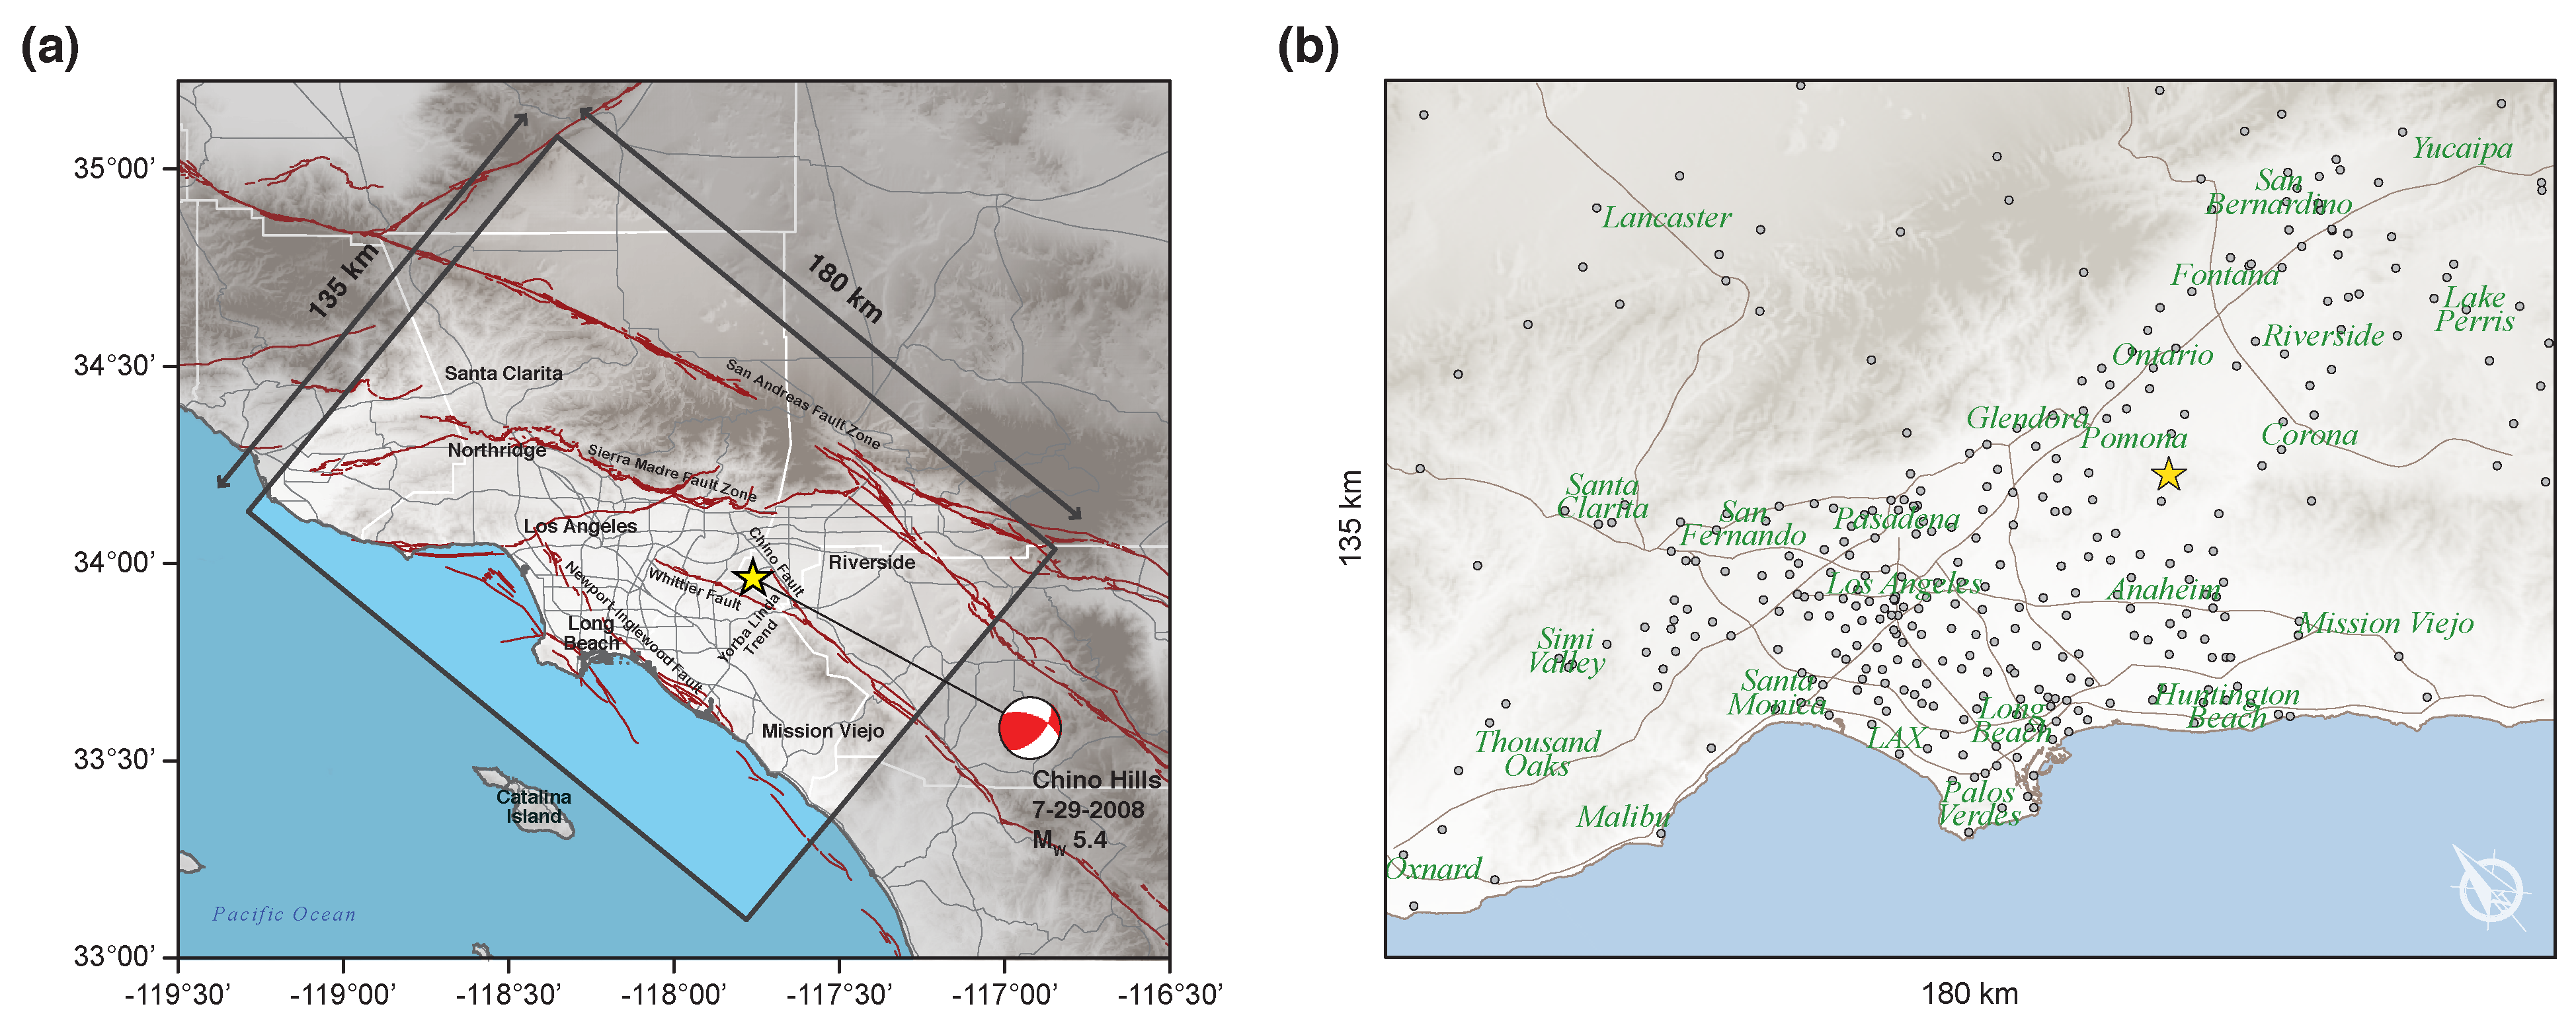
\includegraphics[width=\textwidth]{figures/pdf/figure-01}
    \caption{\textbf{(a)} Region of interest used by \citet{Taborda_2014_BSSA} for the simulations of the 2008 $M_W ~ 5.4$ Chino Hills earthquake, including the epicenter, focal mechanism, and major quaternary faults. In the background, the main roads and topography are shown for visual reference. \textbf{(b)} Distribution of the 336 stations (gray dots) used by \citet{Taborda_2014_BSSA} for the validation analysis of their simulations within the modeling domain shown in part (a). Roads, city names, and the hillshade topography are also shown here in the background for reference. The color version of this figure is available only in the electronic edition.}
    \label{fig:chino-hills}
\end{figure*}

\begin{figure*}[t]
    \centering
    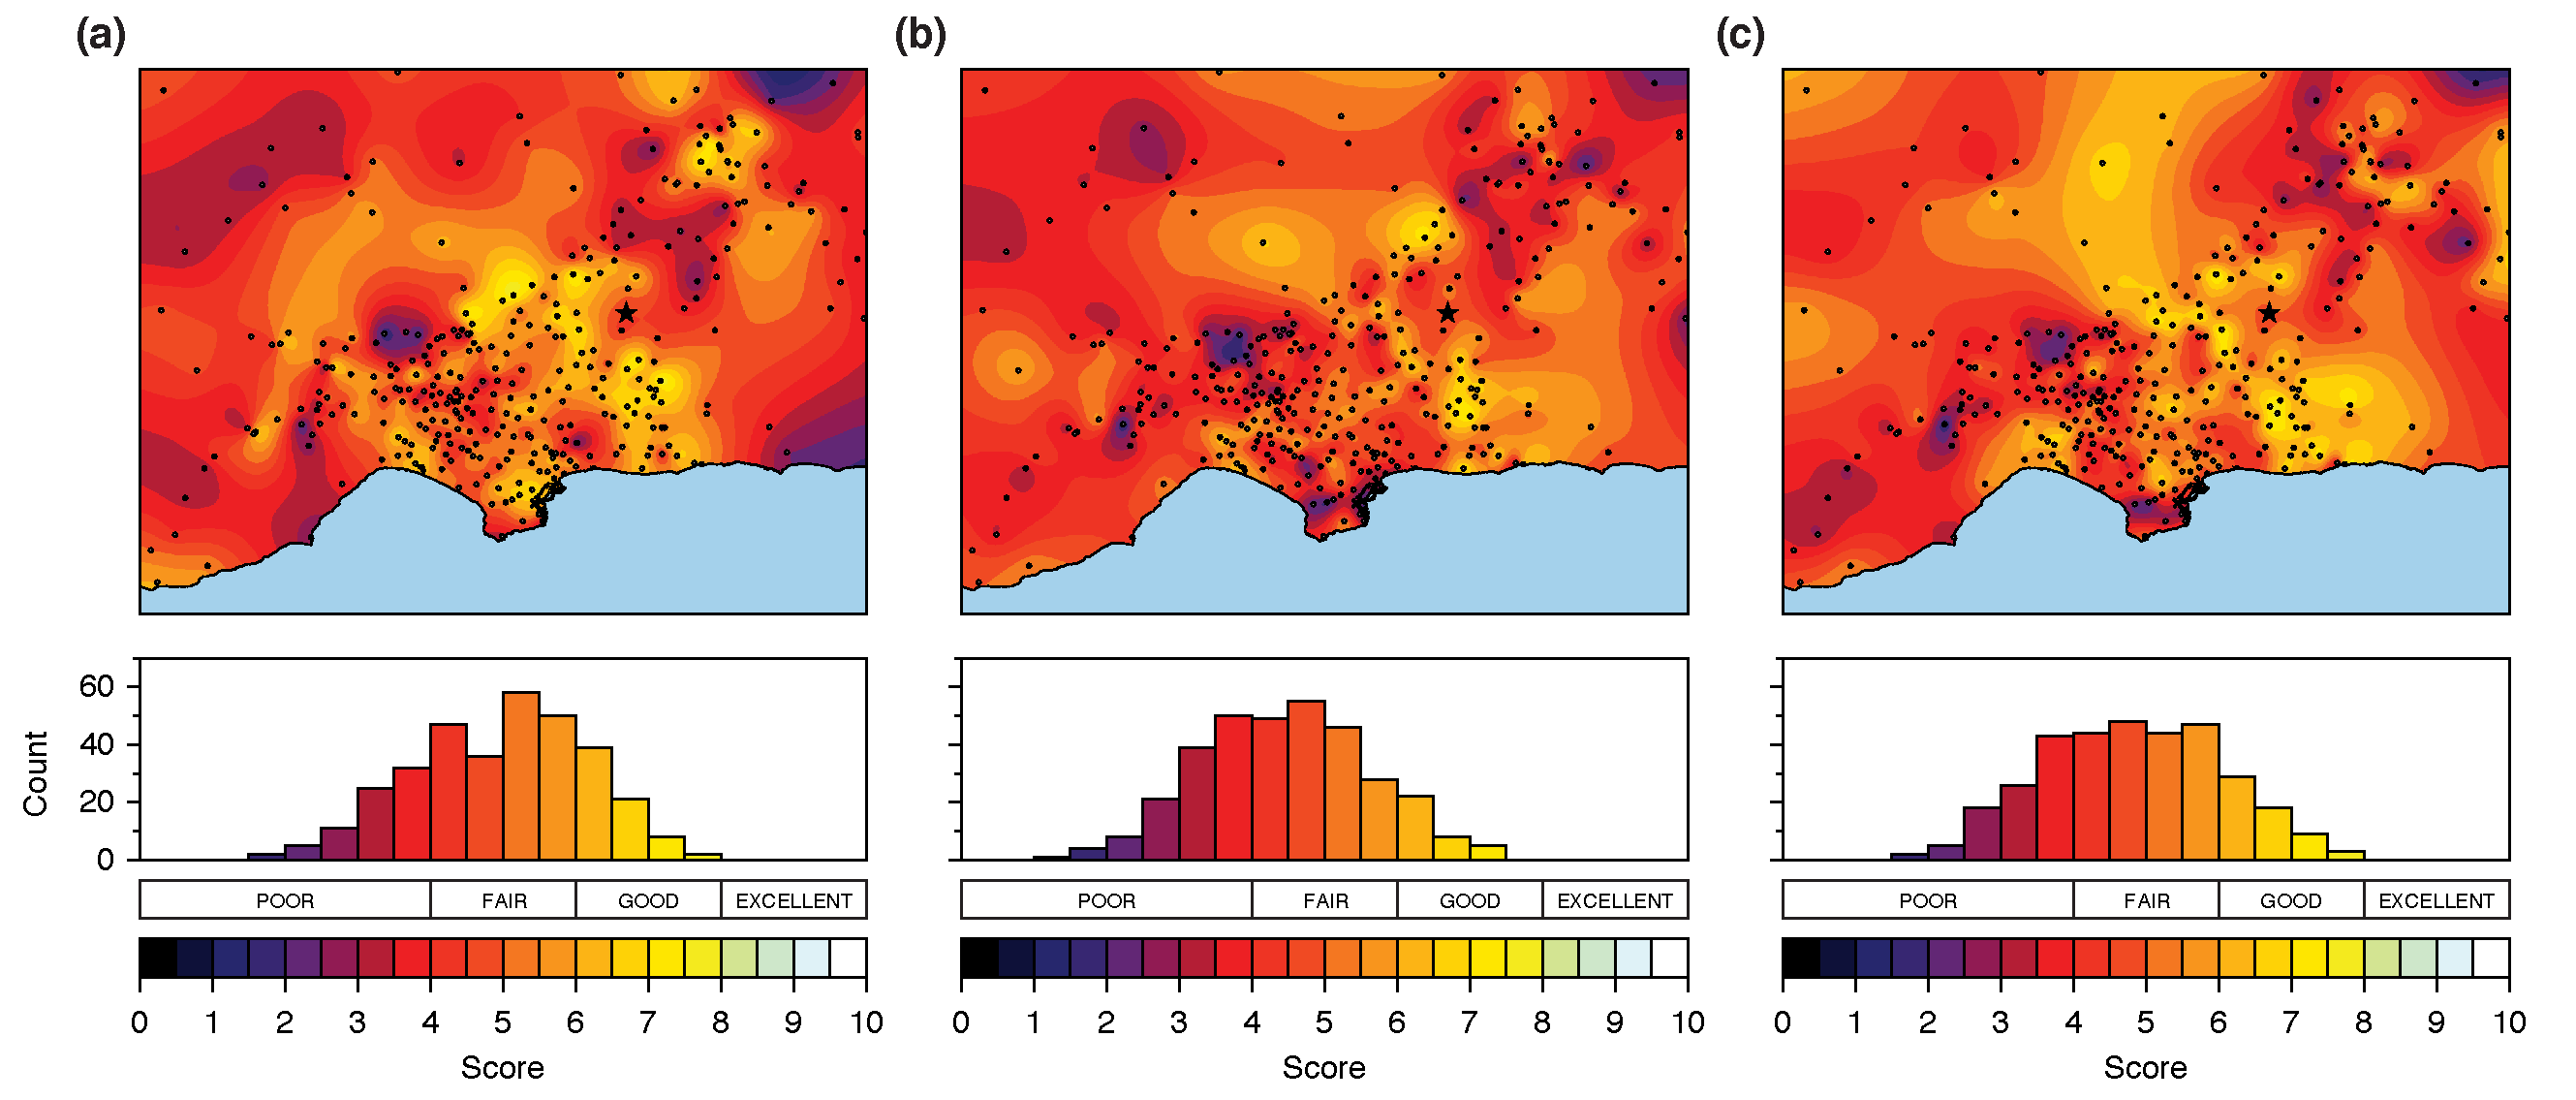
\includegraphics[width=\textwidth]{figures/pdf/figure-02}
    \caption{Validation results obtained by \citet{Taborda_2014_BSSA} in the form of GOF values across the region of interest obtained from comparisons between simulations for three different velocity models and data recorded at ground motion monitoring stations. The distribution of the results at the bottom show the count of stations on the GOF scale defined by \citet{Anderson_2004_Proc} and the ranges of the validation categories: poor, fair, good and excellent. The color version of this figure is available only in the electronic edition.}
    \label{fig:ref-gof-maps}
\end{figure*}

We refer to the set of 11 scores associated with a pair of signals from the work done by \citet{Taborda_2014_BSSA} as one of the \textit{data samples} that compose our dataset. Although at times we will make distinctions between the velocity models and the components of motion for visualization purposes, the clustering analysis to be described in the following section was done using all the data samples in the validation dataset. The motivation behind this choice was that the dataset, as a collection of GOF values, was independent of the simulations and serves here as a generic set of data samples for the purpose of identifying the correlations that exist between the different metrics in Table \ref{tab:metrics}. As such, given the simulations for each velocity model (3), the components of motion (3), and the number of stations used in the validation (336), gave us a large enough dataset, with 3,024 data samples. Figure \ref{fig:data-box-plot} illustrates the idea of a lack of dependence on the simulations by comparing the statistical distribution of the GOF scores of the simulations organized by velocity models and components. It is clear that although there are some differences between them, these are negligible. In other words, the statistical distribution of the data for each metric is about the same independently of model or component. Consequently, and in order to use a dataset as large as possible, we thought it acceptable to combine all the data samples into a single dataset.

\begin{figure}[ht!]
    \centering
    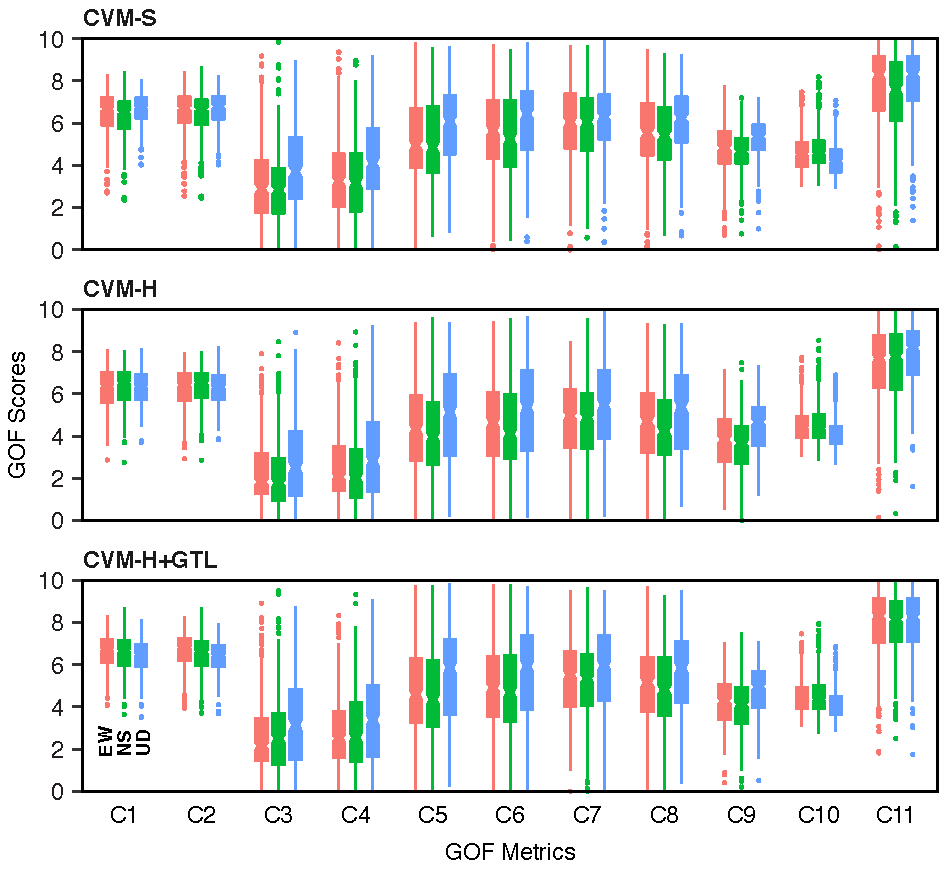
\includegraphics[width=0.48\textwidth]{figures/pdf/figure-03}
    \caption{Statistical distribution of the GOF dataset obtained from \citet{Taborda_2014_BSSA} shown in the form of box-plots for each metric (C1 through C11, see Table \ref{tab:metrics}), velocity model (CVM-S, CVM-H, and CVM-H+GTL), and components of motion (NS, EW, UD). In each case, the boxes represent the interquartile range ($\mathrm{IQR} = \mathrm{Q}3 - \mathrm{Q}1$), the medians are indicated by a notch in the boxes, and the vertical lines show the range of the data, with outliers (data less than $\mathrm{Q}1 - 1.5 \mathrm{IQR}$ and greater than $\mathrm{Q}3 + 1.5 \mathrm{IQR}$) shown as scattered dots. The color version of this figure is available only in the electronic edition.}
    \label{fig:data-box-plot}
\end{figure}
